% This file allows to produce either a separate PDF/PNG image
% See standalone documentation to understand underlying magic

\documentclass[tikz,convert={density=150,size=600,outext=.png}]{standalone}
\usetikzlibrary{shapes, calc, arrows, fit, positioning, decorations, patterns, decorations.pathreplacing, chains, snakes}
% Copyright (c) 2016 Grigory Rechistov <grigory.rechistov@phystech.edu>
% This work is licensed under the Creative Commons Attribution-NonCommercial-ShareAlike 4.0 Worldwide.
% To view a copy of this license, visit http://creativecommons.org/licenses/by-nc-sa/4.0/.

\usepackage{fontspec}
\usepackage{xunicode} % some extra unicode support
\usepackage{xltxtra}

\usepackage{amsfonts}
\usepackage{amsmath}
\usepackage{longtable}
\usepackage{csquotes}

\usepackage{polyglossia}
\setdefaultlanguage[spelling=modern]{russian} % for polyglossia
\setotherlanguage{english} % for polyglossia

% Common settings for all fonts
% 1. Attempt to make fonts be of the same size
% 2. Support TeX ligatures like — = emdash, << >> = guillemets
\defaultfontfeatures{Scale=MatchLowercase, Mapping=tex-text}

% Use Computer Modern Unicode
\newfontfamily\russianfont{CMU Serif}
\setromanfont{CMU Serif}
\setsansfont{CMU Sans Serif}
\setmonofont{CMU Typewriter Text}

% Common packages, commands and their configuration

\newcommand{\abbr}{\textit{англ.}\ }
\newcommand{\todo}[1][]{\textcolor{red}{TODO #1}}


\usepackage{graphicx}
\graphicspath{{pictures/}} % path to pictures, trailing slash is mandatory.

\usepackage{hyperref}
\hypersetup{colorlinks=true, linkcolor=black, filecolor=black, citecolor=black, urlcolor=black , pdfauthor=Grigory Rechistov <grigory.rechistov@phystech.edu>, pdftitle=Программное моделирование вычислительных систем}

\usepackage{footnpag}
\usepackage{indentfirst}
\usepackage{underscore}
\usepackage{url}

\usepackage{listings}
\lstset{basicstyle=\footnotesize\ttfamily, breaklines=true, keepspaces=true }

\usepackage{listings}
\lstset{basicstyle=\footnotesize\ttfamily, breaklines=true, keepspaces=true}

\usepackage{tikz}
\usetikzlibrary{shapes, calc, arrows, fit, positioning, decorations, patterns, decorations.pathreplacing, chains, snakes}
\usepackage{bytefield}

\graphicspath{{../pictures/}} % path to pictures, trailing slash is mandatory.

% The actual drawing follows
\begin{document}
\begin{tikzpicture}[>=latex, font=\small]
    \node[] (gui) {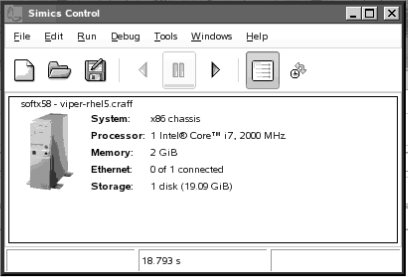
\includegraphics[width=2cm]{./gui.png}};
    \node[above=0.1cm of gui] {Графический интерфейс};
    
    \node[right = 1cm of gui]     (device1) {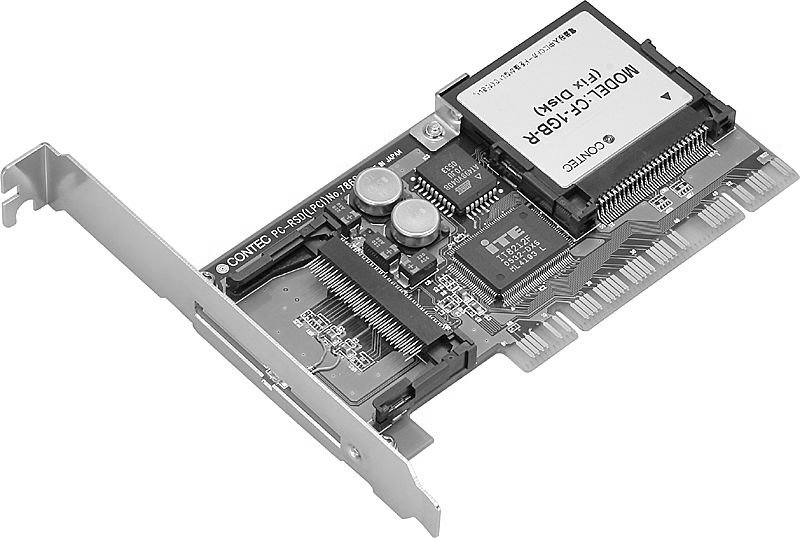
\includegraphics[height=1.5cm]{./device1.png}};
    \node[right = 0.2cm of device1] (device2) {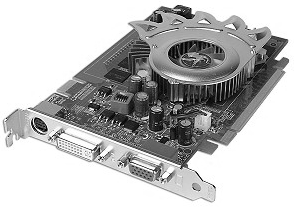
\includegraphics[height=1.5cm]{./device2.png}};
    \node[right = 0.2cm of device2] (device3) {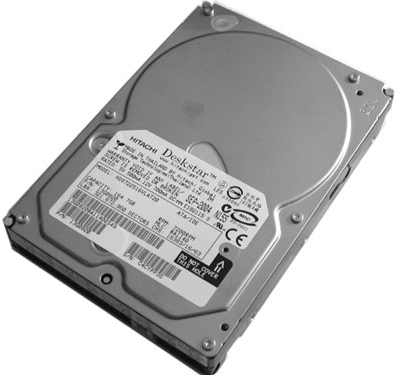
\includegraphics[height=1.5cm]{./device3.png}};
    
    \node[draw, inner sep= 2pt, fit=(device1) (device3)] (frame) {};
    
    \node[below = 2.5cm of gui] (cli) {
\includegraphics[height=1.5cm]{./cli.png}};
    
    \node[draw, circle, below = 0.7cm of device1] (core) {Ядро};
    
    \node[right = 3cm of cli] (python) {
\includegraphics[height=1.5cm]{./python.png}};
    \node[right = 0.2cm of python] (perl) {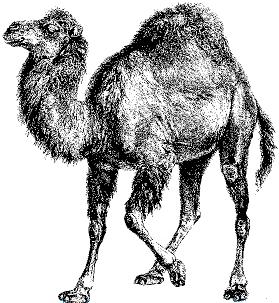
\includegraphics[height=1.5cm]{./perl.png}};
    \node[right = 0.2cm of perl] (lua) {
\includegraphics[height=1.5cm]{./lua.png}};
    
    \node[above=0.1cm of cli] {Командная строка};
    \node[above=0.1cm of perl] {Язык сценариев};
    \node[above=0.1cm of device2] {Модели устройств};
    
    \draw[<->, shorten >=0.8cm] (core) -- (gui);
    \draw[<->, shorten >=0.2cm] (core) -- (frame);
    \draw[<->, shorten >=0.8cm] (core) -- (cli);
    \draw[<->, shorten >=0.8cm] (core) -- (perl);
\end{tikzpicture}


\end{document}
